\subsection{Measurement of Dropbox Performance Metrics}\label{sec:application:cloud_file_synchronisation:application_measurements}
The model presented in \refsec{sec:application:cloud_file_synchronisation:system_model} requires several input parameters which are obtained from measurements and described in this section.
First, we give an overview over the measurement setup implemented in the distributed testbed PlanetLab~\cite{Chun2003}.
Then, we present measurement results as well as fitted distributions for both up and download bandwidth as well as for the time used by the cloud service to prepare data prior to the download.
Finally, we derive a image file size distribution by analysing a large set of digital photos.

\subsubsection*{Bandwidth and Preparation Times}\label{sec:application:cloud_file_synchronisation:application_measurements:bandwidth_preparation_times}
We obtain a PlanetLab slice containing all momentarily available nodes in February 2014 and discard every node not responding to \texttt{ping} or \texttt{ssh} within a \SI{20}{\second} interval.
On the remaining \(87\) nodes we install our measurement setup.
This includes two instances of the \dropbox client on each host, linking them to a specially created \dropbox account and two different directories.
Furthermore, we disable the \emph{LAN-Synchronisation} feature for both clients.
After ensuring that both shared directories are empty, we create a file with randomly generated content of \SI{10}{\mega\bit} size, unique per node.
Files are unique in order to compensate for caching algorithms by \dropbox, as the client calculates a checksum of the file prior to uploading and only uploads the file if no duplicate file is already stored in the account, in order to conserve bandwidth.
Further, the randomly generated content ensures that no significant compression results can be achieved before uploading, resulting in comparable results for the time required to upload the files.
After the file is created, we start \texttt{tcpdump} and \emph{symlink} the file to the first directory shared via \dropbox while taking note of the \emph{initial timestamp} of the symlink.
As the complete file has finished downloading and appears in the second \dropbox directory, we note the current \emph{final timestamp} and stop \texttt{tcpdump}.
Finally, we retrieve the traffic dump and the recorded timestamps and reset the measurement setup.

\begin{figure}
  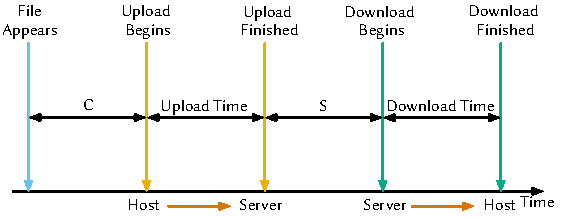
\includegraphics{application/cloud_file_synchronization/application_measurements/figures/measurement_setup}
  \caption{Setup used to peform measurement.}
  \label{fig:application:cloud_file_synchronisation:application_measurements:bandwidth_preparation_times:measurement_setup}
\end{figure}

This process is repeated \(8\) times for all available PlanetLab nodes.
Based on the two recorded timestamps as well as the traffic dump, we calculate the required values for the model as shown in \reffig{fig:application:cloud_file_synchronisation:application_measurements:bandwidth_preparation_times:measurement_setup}.
The time between the \emph{initial timestamp} and the first packet sent to the \emph{Amazon S3} storage server is considered the client preparation time \clientpreparationtime.


The upload time \(t_u\) is given by the time between the first and the last packet uploaded to the storage server and is used to calculate the mean upload bandwidth \(\uploadbandwidth = \SI{10}{\mega\bit} / t_u.\)
The server preparation time \serverpreparationtime is given by the time between the last packet uploaded and the first packet downloaded from the storage server.
Finally, we calculate the mean download bandwidth \downloadbandwidth similar to the upload bandwidth by considering the time between the first downstream packet from the storage server and the completion of the file download.

\begin{figure}
  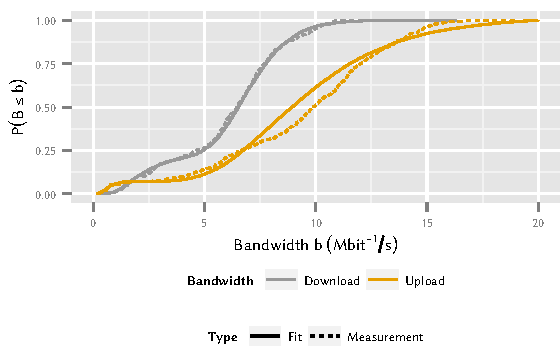
\includegraphics{application/cloud_file_synchronization/application_measurements/figures/bandwidths}
  \caption{Measurement and corresponding fit for upload bandwidth \uploadbandwidth and download bandwidth \downloadbandwidth.}
  \label{fig:application:cloud_file_synchronisation:application_measurements:bandwidth_preparation_times:measurement_setup:bandwidths}
\end{figure}

In \reffig{fig:application:cloud_file_synchronisation:application_measurements:bandwidth_preparation_times:measurement_setup:bandwidths} we show the mean upload and download bandwidth obtained from our measurements, as well as fitted distributions.
For the fit we considered a set of different possible distributions, including exponential, log-normal, gamma, Pareto, and Weibull.
We found that none of the considered distributions provided an adequate fit due to the slope at the \SI{7}{\percent} quantile for the upload, respectively \SI{25}{\percent} quantile for the download bandwidth.
To adapt for this behaviour, we consider a \emph{$2$-hyper log-normal} distribution \cite{Wang2006} with partitions at \(0.07\) or \({0.25}\).
After splitting, the random variables are fitted to log-normal random variables using \texttt{fitdistrplus}\footnote{\url{https://cran.r-project.org/web/packages/fitdistrplus}, \accessed} for the \emph{R} language.
The resulting parameters for the upload bandwidth \uploadbandwidth and download bandwidth \downloadbandwidth can be found in \reftab{tab:application:cloud_file_synchronisation:application_measurements:bandwidth_preparation_times:measurement_setup:fit}, where \(\mu_1\) and \(\sigma_1\) are the location and scale parameters for the \emph{lower} part of the compound distribution and \(\mu_2\) and \(\sigma_2\) are the location and scale of the \emph{upper} part of the compound distribution.

\begin{table}
  \centering
  \begin{tabular}{lccccc}
    \toprule
    Random variable&Split&\(\mu_1\)&\(\sigma_1\)&\(\mu_2\)&\(\sigma_2\)\\
    \midrule
    \uploadbandwidth & 0.07 & 13.44 & 0.49 & 16.10 & 0.37\\
    \downloadbandwidth & 0.23 & 14.63 & 0.51 & 15.81 & 0.21 \\
    \serverpreparationtime & -- & 1.35 & 0.41 & -- & --\\
    \imageFileSize & 0.35 & 14.17 & 0.54 & 15.24 & 0.33 \\
    \bottomrule
  \end{tabular}
  \caption{Distribution parameters for considered random variables.}
  \label{tab:application:cloud_file_synchronisation:application_measurements:bandwidth_preparation_times:measurement_setup:fit}.
\end{table}


\begin{figure}
  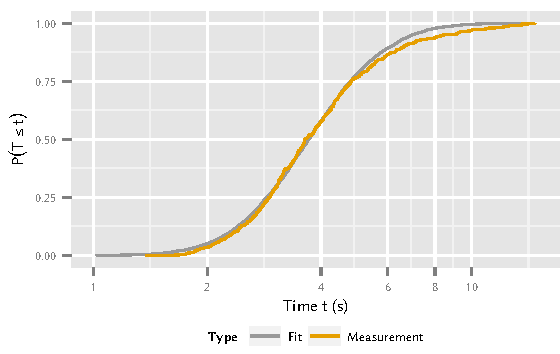
\includegraphics{application/cloud_file_synchronization/application_measurements/figures/server_preparation_time}
  \caption{Measurement and fit of server preparation time \serverpreparationtime.}
  \label{fig:application:cloud_file_synchronisation:application_measurements:bandwidth_preparation_times:measurement_setup:server_preparation_time}
\end{figure}

Next, we consider the client and server preparation times.
As our intent is to evaluate the performance of different scheduling mechanisms for the upload phase, we require only the amount of time \clientpreparationtime used for computing hashes of the files considered for upload without considering the time used by the scheduling mechanism.
To obtain an approximation, we use the \emph{minimum} of all observed upload preparation phases \(\clientpreparationtime = \SI{1.32}{\second}\).
For the server preparation time \serverpreparationtime we obtain a fit, finding that a Log-normal distribution provides the best result of the considered distributions, as shown in \reffig{fig:application:cloud_file_synchronisation:application_measurements:bandwidth_preparation_times:measurement_setup:server_preparation_time}.
The parameters of the resulting distribution are given in \reftab{tab:application:cloud_file_synchronisation:application_measurements:bandwidth_preparation_times:measurement_setup:fit}.

\begin{figure}
  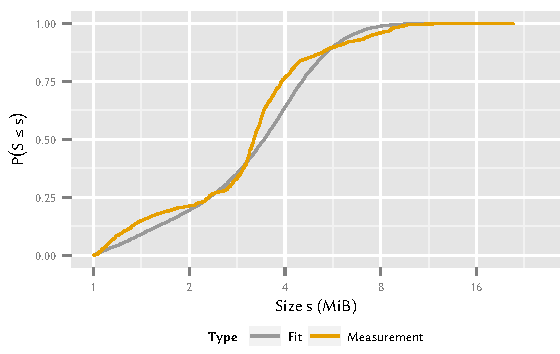
\includegraphics{application/cloud_file_synchronization/application_measurements/figures/image_size}
  \caption{Image file size distribution \imageFileSize and corresponding fit.}
  \label{fig:application:cloud_file_synchronisation:application_measurements:bandwidth_preparation_times:measurement_setup:image_size}
\end{figure}

\subsubsection*{Image File Sizes}\label{sec:application:cloud_file_synchronisation:application_measurements:image_file_sizes}
In order to obtain a representative random variable for the size of image files, we evaluate a set of \({1375}\) pictures of varying image quality taken by different cameras.
We record the file-size and evaluate the quality of fits using different random variables as shown in~\reffig{fig:application:cloud_file_synchronisation:application_measurements:bandwidth_preparation_times:measurement_setup:image_size}.
We find that similar to the upload and download bandwidth, a \(2\)-Hyper Log-normal distribution provides best results and present the distribution parameters in \reftab{tab:application:cloud_file_synchronisation:application_measurements:bandwidth_preparation_times:measurement_setup:fit}.

